\begin{frame}{Double objectif}
	\begin{figure}
		\centering
		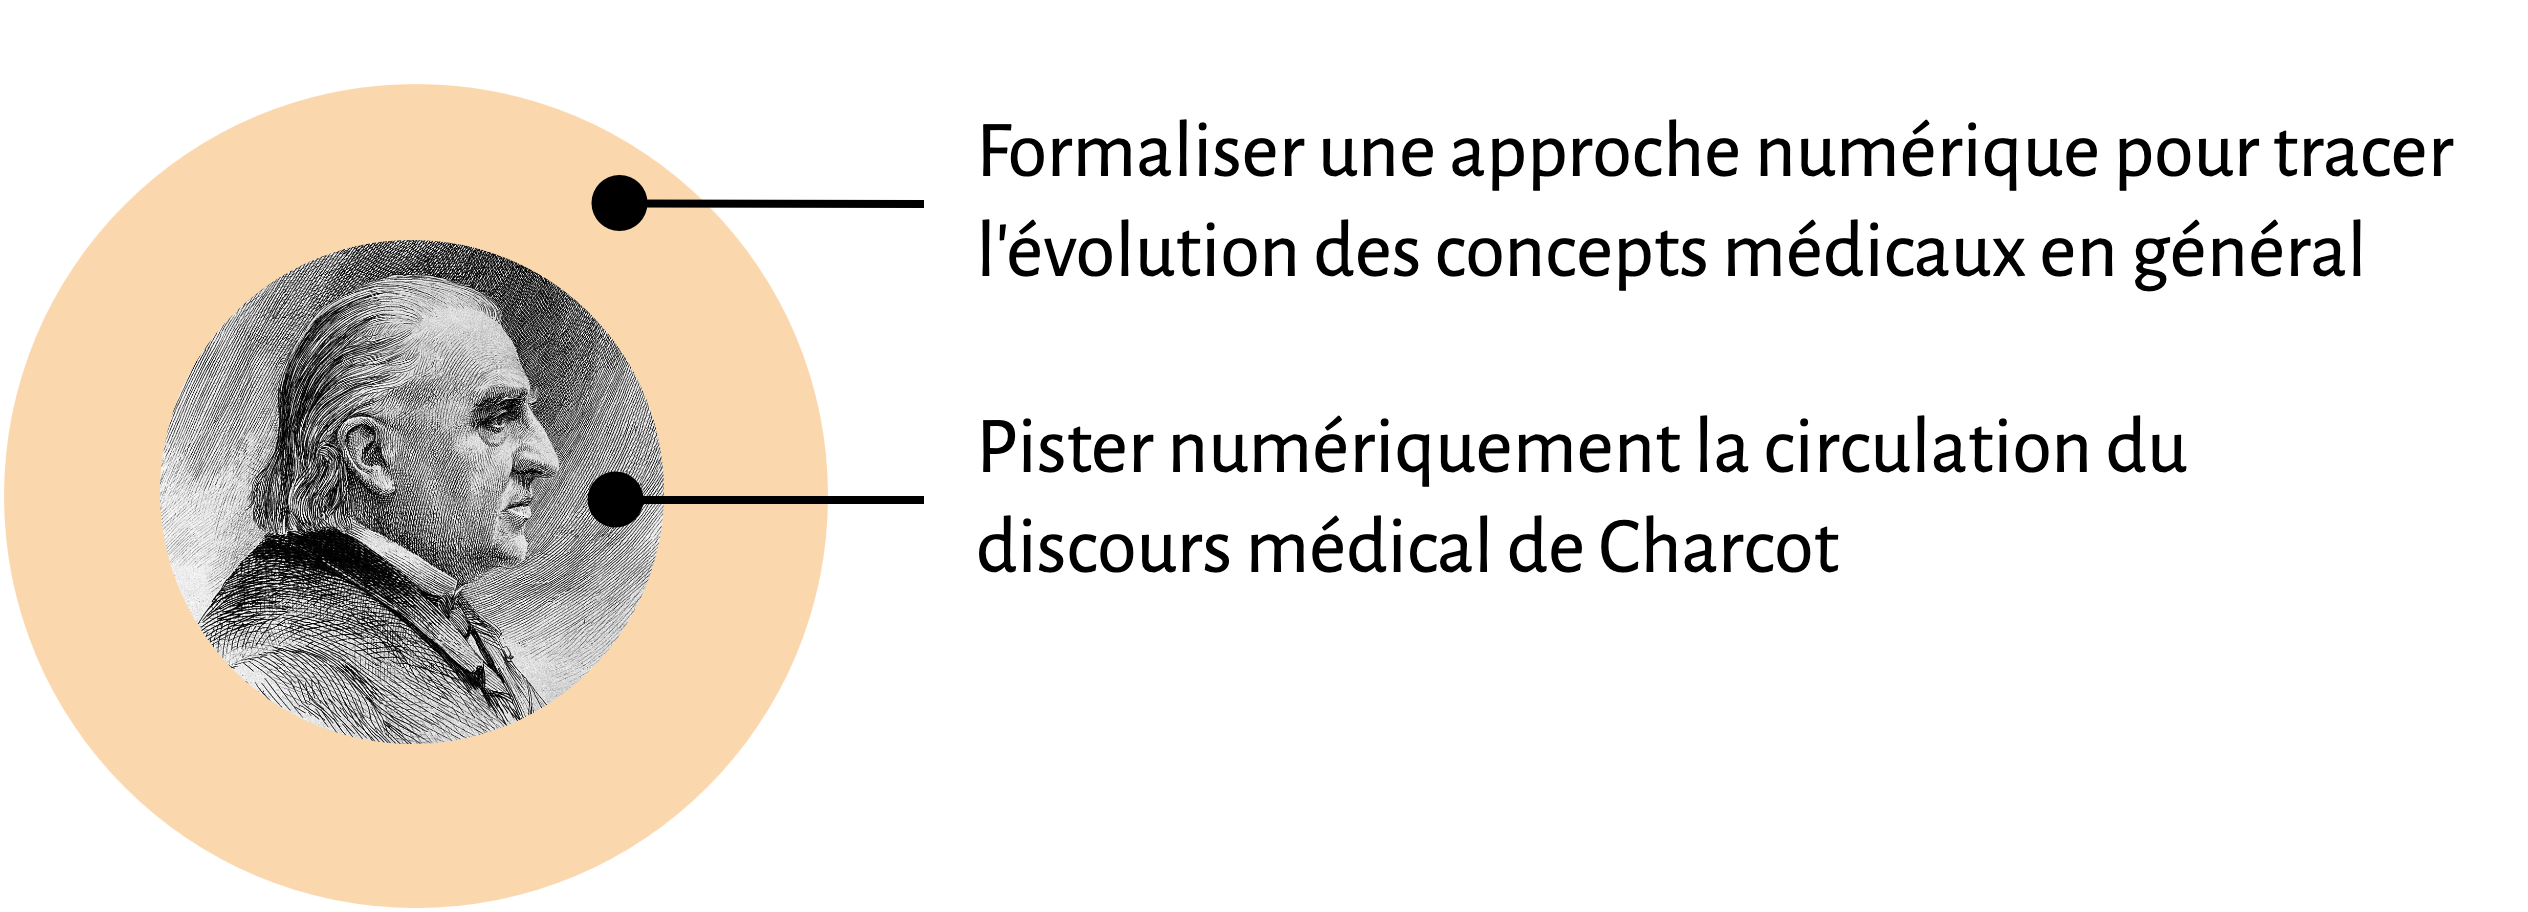
\includegraphics[width=1\textwidth]{pic/objectif_double.png}
		%\caption{}
	\end{figure}
	
	\begin{variableblock}{}{bg=white,fg=red}{bg=green,fg=pink}
		\centering
		Est-il possible de mesurer l'impact de Charcot sur son réseau scientifique\textcolor{BlueViolet}{*} en s'appuyant sur les termes scientifiques qu'il a employés ?
	\end{variableblock}
	\begin{flushright}
		{\footnotesize\textcolor{BlueViolet}{* élèves, collègues et successeurs\\
				$\rightarrow$ collaborateurs}}
	\end{flushright}
	
	
\end{frame}

\begin{frame}{Hypothèses}


	\begin{variableblock}{}{bg=white,fg=deepblue}{bg=green,fg=pink}
		\justifying
	Le texte comme point d’entrée pour étudier les tendances de la circulation des idées à l'aide des caractéristiques structurelles spécifiques \\\raggedleft\textcolor{deepred}{\citep{milia2023}}
\end{variableblock}

		\begin{variableblock}{}{bg=white,fg=deepblue}{bg=green,fg=pink}
	\justifying
	Certains \textbf{termes médicaux} dont Charcot a été l’inventeur (\textsc{SLA}) ou le transmetteur (\textit{hystérie}) ont été repris de manière significative dans les écrits de son réseau scientifique.
\end{variableblock}
\end{frame}

\begin{frame}{Recherches quantitatives des circulations des savoirs}
	%Domaine peu documenté
	Tendances de circulation linguistique dans les fronts de recherche 

	
			        \begin{figure}[!h]
		\centering
		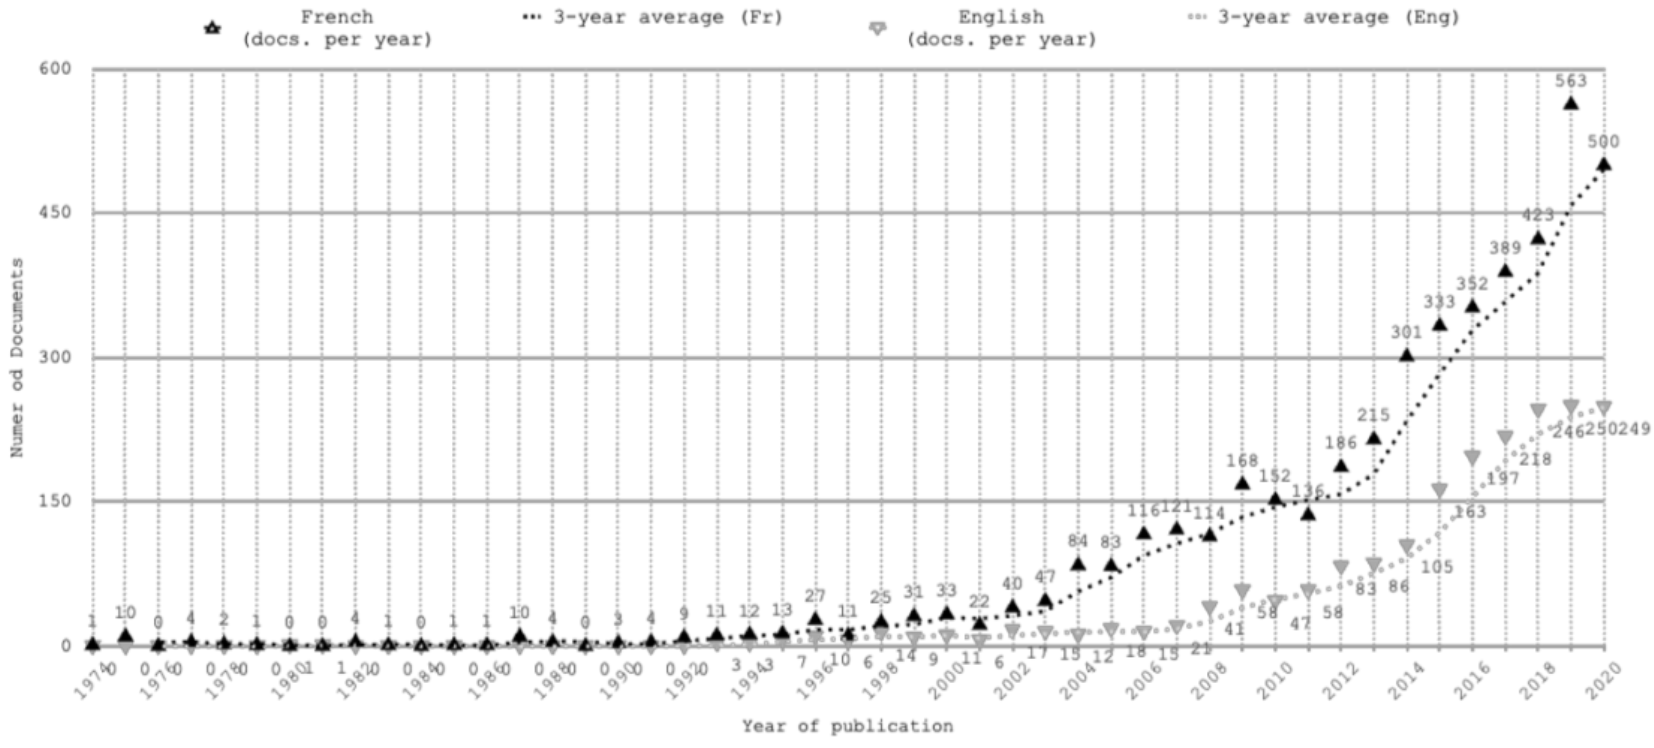
\includegraphics[width=1\textwidth]{pic/thematic_interests.png}
		\caption{Nombre de documents représentant les intérêts thématiques en anglais et en français \citep{milia2023}.}
	\end{figure}
	
\end{frame}


\begin{frame}{Recherches quantitatives des circulations des savoirs}
	%Domaine peu documenté
	Tendances de circulation linguistique dans les fronts de recherche 
	
	
	\begin{figure}[!h]
		\centering
		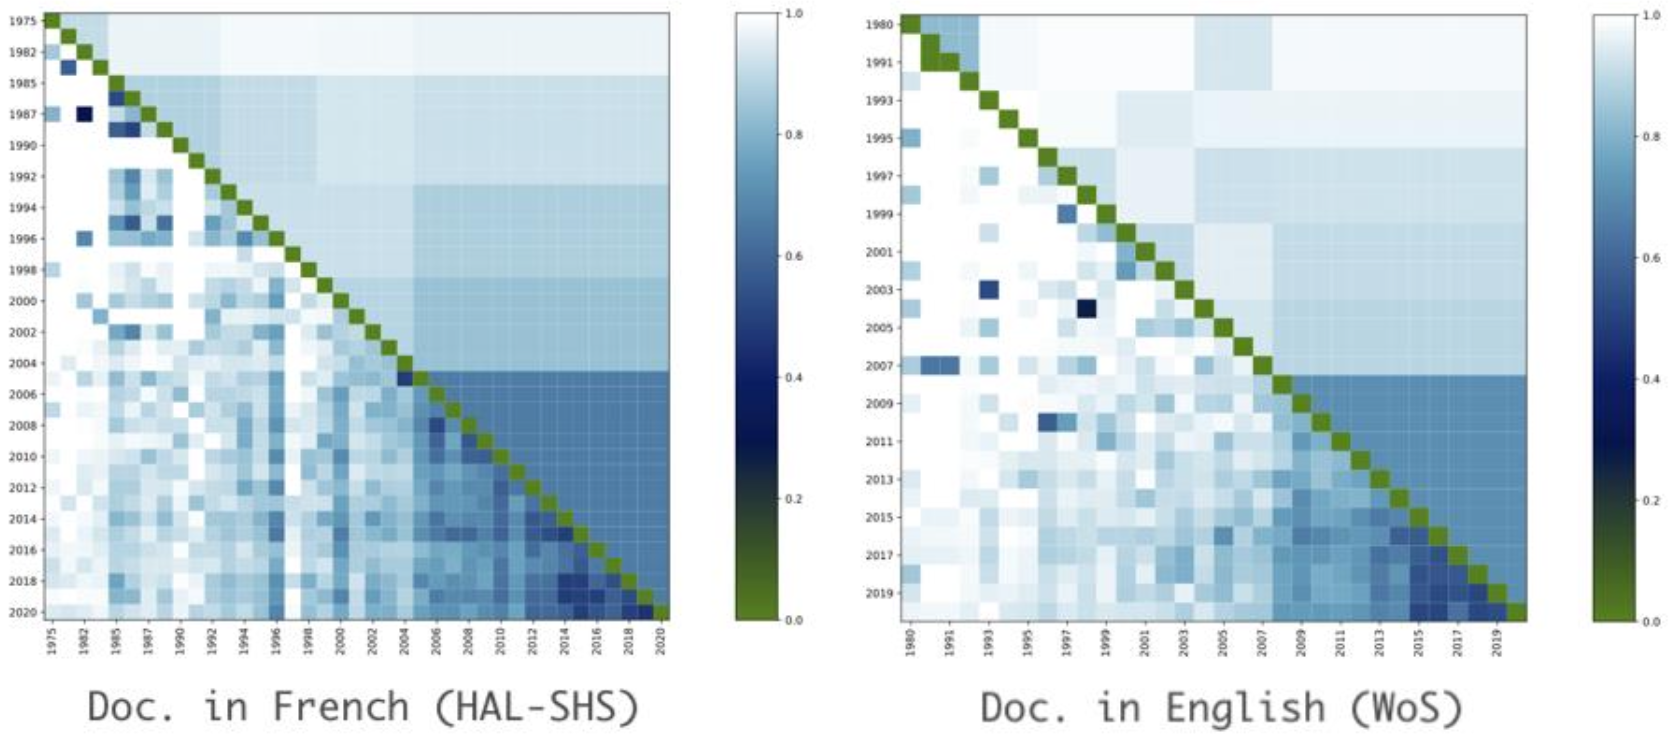
\includegraphics[width=1\textwidth]{pic/period_detection.png}
		\caption{Détection de période à l'aide d'une corrélation significative des termes au fil des années dans deux sources et langues différentes \citep{milia2023}.}
	\end{figure}
	
\end{frame}



\begin{frame}{Recherches quantitatives des circulations des savoirs}
	\begin{itemize}
	\item réception de la pensée scientifique de C. Bernard \citep{riguet2018impact}
\item détection des réemplois textuels
\citep{fedchenko2024recherche}
\item Rankingdom -- mesurer l'importance d’une entité \citep{soulet2024}
\end{itemize}
\begin{figure}[!h]
\centering
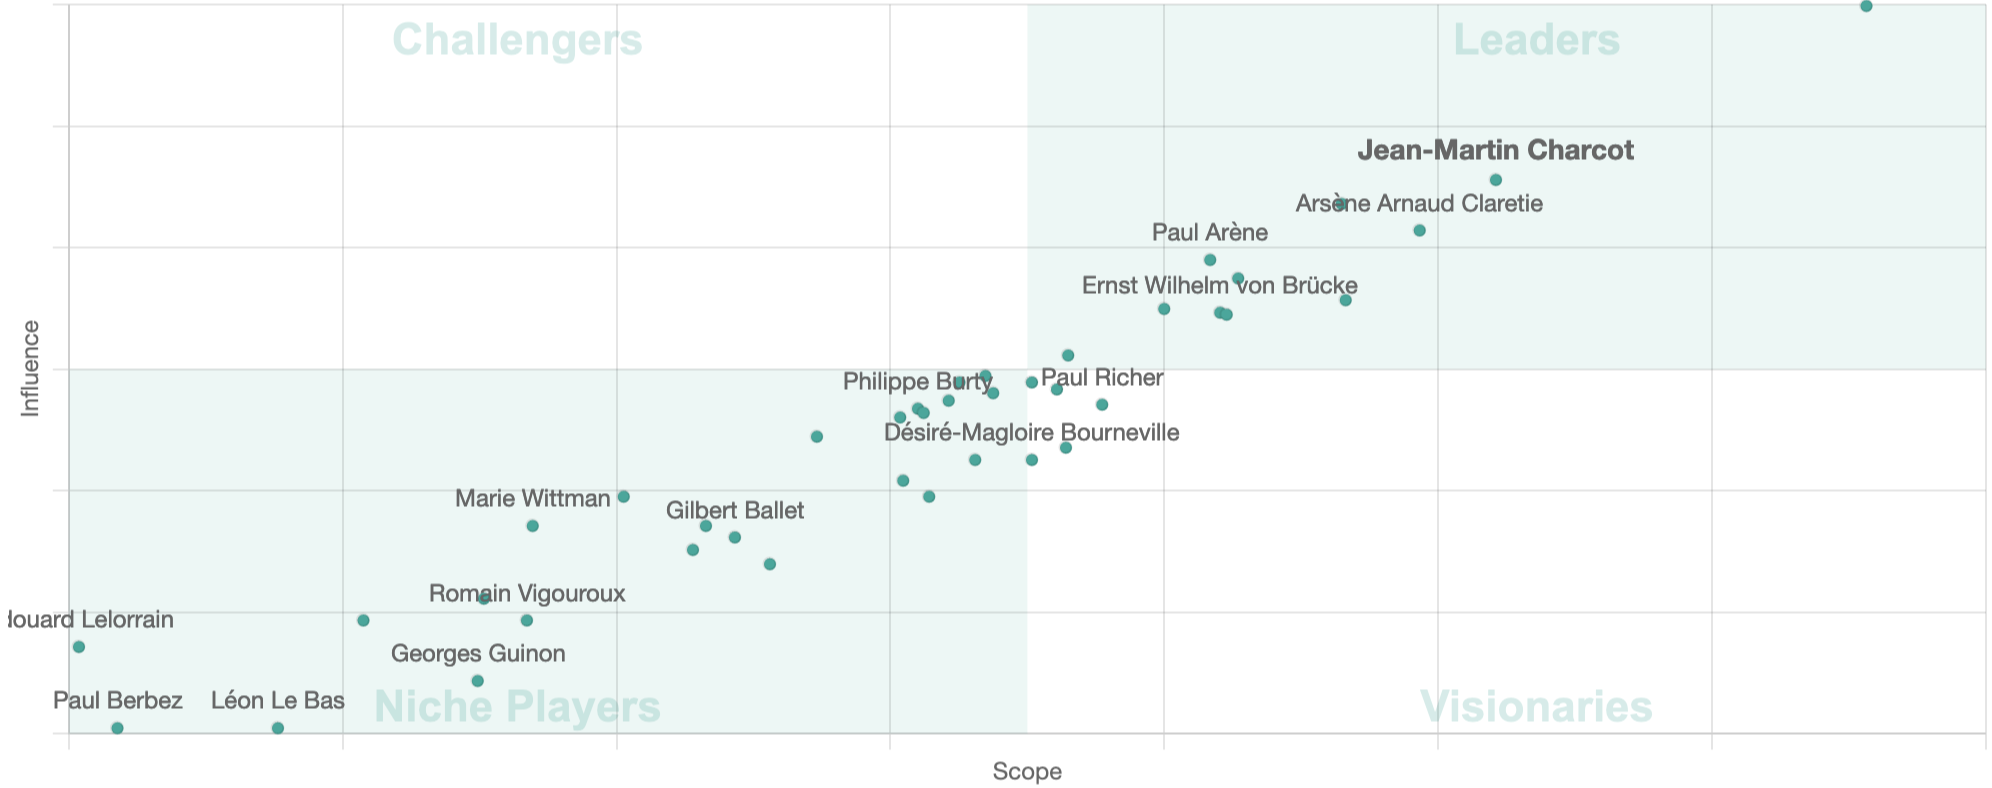
\includegraphics[width=1\textwidth]{pic/analyse_quadrant.png}
\caption{Positionnement de l'entité \texttt{Charcot} au sein de son domaine \textit{via} l'analyse de quadrant.}
\end{figure}
\end{frame}

%\begin{frame}{Impact temporel de Charcot}
%\begin{figure}[!h]
%		\centering
%		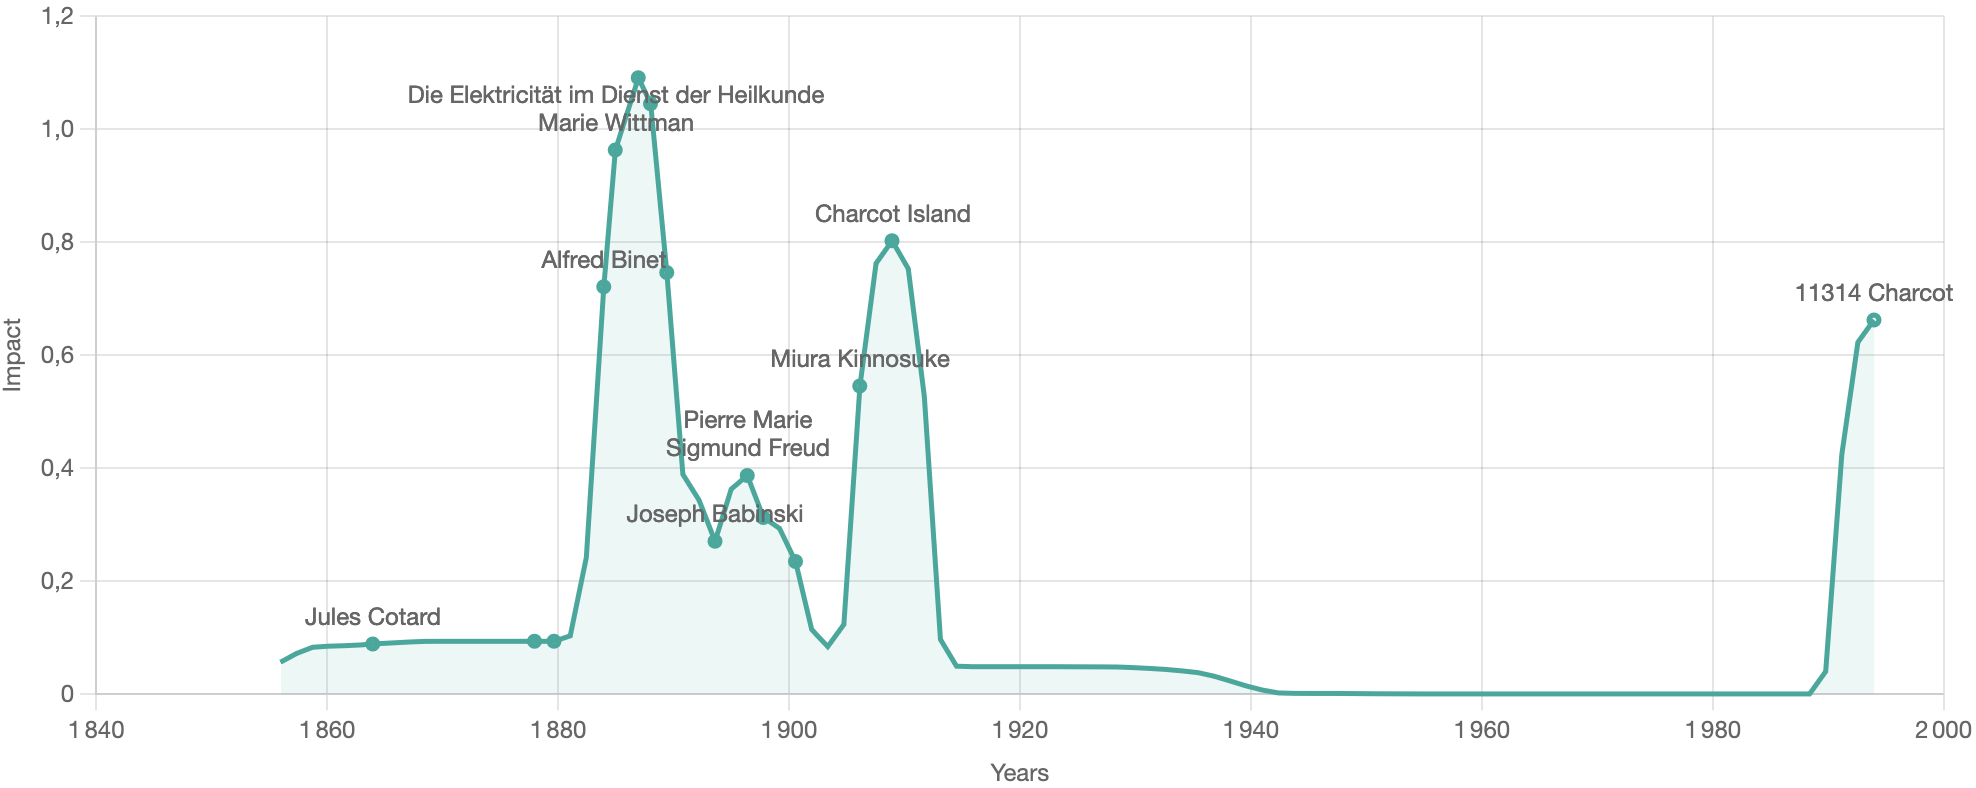
\includegraphics[width=1\textwidth]{pic/impact_temporel.png}
%		\caption{Analyse temporelle de l'impact de l'entité \texttt{Charcot} \textit{via} Rankingdom.}
%	\end{figure}
%\end{frame}



